\documentclass{article}
\usepackage[utf8]{inputenc}
\usepackage[colorinlistoftodos]{todonotes}
\usepackage{setspace}
\usepackage[margin = 1in]{geometry}
\usepackage{amsmath}
\usepackage[
    backend=biber,
    style=authoryear,
    natbib=true,
    url=true, 
    doi=true,
    eprint=true
]{biblatex}
\addbibresource{research.bib}
\usepackage{graphicx}
\usepackage{subcaption}
\usepackage{array}



\usepackage{hyperref}
\hypersetup{
    colorlinks=true
}


\title{Chapter 3B}
\author{Frederick Boehm}
\date{\today}

\begin{document}
\doublespacing
\maketitle
\listoftodos
\tableofcontents
\listoffigures
\listoftables



\section{Introduction}

The goal of this section is to characterize the statistical power of our pleiotropy vs. separate QTL test under a variety of conditions by studying a real data set. We examine pancreatic islet expression traits from the \citet{keller2018genetic} data. As in chapters 2 and 3A, we test only two traits at a time. Because we’ve chosen local expression traits in our analysis, we both know where each trait’s true QTL location (approximately), and we anticipate that each trait has a unique QTL that is distinct from QTL for other local expression traits. This design thus provides opportunities to study statistical power for our test.

We anticipate that inter-locus distance, univariate QTL strength, and correlation of founder allele effects patterns are three factors that contribute to power for our test. Specifically, we expect that greater inter-locus distance, greater univariate LOD peak heights, and less similar founder allele effects patterns correspond to greater statistical power to detect two separate QTL. 

We use pancreatic islet gene expression traits from a publicly available data set, which \citet{keller2018genetic} first collected, analyzed, and shared. We examine a collection of 80 local traits on Chromosome 19 and perform our test for pleiotropy vs. separate QTL on pairs of traits. We also examine pairwise relationships among gene expression traits to characterize the impacts of univariate LOD peak height, inter-locus distance, and similarity of founder allele effects patterns on pleiotropy vs. separate QTL test statistic values.



\section{Methods}

\subsection{Data description}

We analyzed data from 378 Diversity Outbred mice \citep{keller2018genetic}. \citet{keller2018genetic} genotyped tail biopsies with the GigaMUGA microarray \citep{morgan2016mouse}. They also used RNA sequencing to measure genome-wide pancreatic islet cell gene expression for each mouse at the time of sacrifice \citep{keller2018genetic}. They shared these data, together with inferred founder allele probabilities, on the Data Dryad site (\url{https://datadryad.org/resource/doi:10.5061/dryad.pj105}). 

We downloaded the file "Attie\_DO378\_eQTL\_viewer\_v1.Rdata" from Data Dryad \citep{keller2018genetic} and analyzed the data in the R statistical computing environment \citep{r}. We used the R packages \texttt{qtl2} \citep{broman2018} and \texttt{qtl2pleio} \citep{qtl2pleio} in our analyses. 

\subsection{Study design}

We focus on 80 local expression QTL and their corresponding transcript levels. We define a local expression QTL to be an expression QTL that is on the same chromosome as the gene itself. For example, the \emph{Asah2} gene is located on Chromosome 19 and its transcript levels have an expression QTL on Chromosome 19 (Table \ref{tab:ann4}). Thus, we term the Chromosome 19 \emph{Asah2} expression QTL a local expression QTL. 

We choose to focus on local expression QTL, while ignoring nonlocal expression QTL, because we know, approximately, the true locations for local expression QTL. That is, a local expression QTL is near the corresponding gene position. Additionally, we expect that a given local expression QTL affects only one local expression trait. In our example above, we expect that the \emph{Asah2} expression QTL is near the \emph{Asah2} gene position and that no other local expression traits map to it.


Our design involves selection of a set of ``anchor'' expression traits. Gene \emph{Asah2} is located near the center of Chromosome 19 and has a very strong local expression QTL (Table \ref{tab:ann4}). We chose it as our first ``anchor'' gene expression trait. To diversify our collection of anchor genes, we chose three additional expression traits with local expression QTL. These three are Lipo1, Lipo2, and 4933413C19Rik (Table \ref{tab:ann4}). Together, the four anchor genes represent a variety of local expression trait LOD peak heights (from 60 to 101) and demonstrate modest variability in their founder allele effects patterns (Figure \ref{fig:founder-allele-effects}). All four anchor genes are located near the middle of Chromosome 19.  




We identified a set of 76 non-anchor local expression traits that map to the 20-Mb region centered on the peak for \emph{Asah2}, at 32.1 Mb. Each trait among the 76 maps to Chromosome 19 with a univariate LOD of at least 10 (Table \ref{tab:ann76}). 


% latex table generated in R 3.5.2 by xtable 1.8-3 package
% Thu Jan  3 16:29:15 2019
\begin{table}[ht]
\centering
\begin{tabular}{>{\em}lrrrr}
  \hline
symbol & start & end & peak\_position & lod \\ 
  \hline
Asah2 & 31.98 & 32.06 & 32.14 & 101.20 \\ 
  Lipo1 & 33.52 & 33.76 & 33.67 & 85.46 \\ 
  Lipo2 & 33.72 & 33.76 & 33.02 & 77.21 \\ 
  4933413C19Rik & 28.58 & 28.58 & 28.78 & 60.41 \\ 
   \hline
\end{tabular}
\caption{Annotations for four anchor genes.}\label{tab:ann4}
\end{table}





\subsection{Univariate QTL LOD calculations}

\citet{keller2018genetic} shared univariate QTL mapping results in their file on Data Dryad. For a given univariate QTL scan, they fitted the following linear mixed effects model at every marker:

\begin{equation}\label{eq:lmm}
Y = XB + WC + G + E
\end{equation}

\noindent where $Y$ is a $n$ by $1$ matrix containing measured values for a single phenotype, $X$ is a $n$ by $8$ matrix of founder allele dosages for a single marker, $B$ is a $8$ by $1$ matrix of founder allele effects, $W$ is a $n$ by $4$ matrix of covariates (sex and three wave indicators), $C$ is a $4$ by $1$ matrix of covariate effects, $G$ is a $n$ by $1$ matrix of polygenic random effects, and $E$ is a $n$ by $1$ matrix of random errors. They also assumed that $G$ and $E$ are independent and that 

\begin{equation}\label{eq:uniG}
G \sim N(0, \sigma_g^2K)
\end{equation}

\begin{equation}\label{eq:uniE}
E \sim N(0, \sigma_e^2I)
\end{equation}


The model fitting procedure involves first an expectation - maximization algorithm to estimate the variance components with restricted maximum likelihood \citep{broman2018}. The model above is fitted, but without genotype data. A column of $1$'s replaces the $n$ by $8$ matrix of founder allele probabilities. Thus, variance components are estimated only once for each trait.

\citet{keller2018genetic} then used generalized least squares to fit the models with genotype data (Equation \ref{eq:uni-Bhat}). Implicitly, this procedure assumes that the covariance matrix does not depend on the genotype data. The R package \texttt{qtl2} implements these calculations \citep{broman2018}. 

\subsection{Estimating founder allele effects}

For each Chromosome 19 marker, we estimated founder allele effects from the model above (Equations \ref{eq:lmm}, \ref{eq:uniG}, \ref{eq:uniE}. We calculated:

\begin{equation}\label{eq:uni-Bhat}
\widehat {(B:C)} = \left((X:W)^T\hat\Gamma^{-1}(X:W)\right)^{-1}(X:W)^T\hat\Gamma^{-1}Y
\end{equation}

\noindent where $B:C$ denotes the concatenation of $B$ and $C$, and $X:W$ refers to the $n$ by $12$ matrix resulting from appending the columns of $W$ to the $X$ matrix. $\hat\Gamma$ is the covariance matrix defined by Equation \ref{eq:Sigma}.

\begin{equation}\label{eq:Sigma}
\hat \Gamma = \hat\sigma_g^2 K + \hat \sigma_e^2 I_n
\end{equation}

\noindent We denote the restricted maximum likelihood estimates of the variance components by $\hat \sigma_g^2$ and $\hat \sigma_e^2$. 



\subsection{Two-dimensional QTL scans}

We performed two-dimensional QTL scans for $4 * 76 + \binom{4}{2} = 310$ pairs. Each pair included one of the four "anchor" gene expression traits and either one of 76 non-anchor gene expression traits or one of the remaining three anchor gene expression traits. 

Our two-dimensional QTL scan encompassed a 1000 by 1000 marker grid from 18.1 Mb to 42.5 Mb on Chromosome 19. Each scan involved fitting 1000 x 1000 = 1,000,000 linear models via generalized least squares after first estimating the variance components for the model without genotype data. For a given ordered pair of markers, we used the model defined by Equations \ref{eq:mvlmm}, \ref{eq:mvG} and \ref{eq:mvE}.

\begin{equation}
vec(Y) = Xvec(B) + vec(G) + vec(E)
\label{eq:mvlmm}
\end{equation}

where $Y$ is a $n$ by $2$ matrix containing measurements for two traits on each of $n$ mice, $B$ is a $12$ by $2$ matrix of effects for the eight founder alleles and four covariates, $G$ is a $n$ by $2$ matrix of polygenic random effects, and $E$ is a $n$ by $2$ matrix of random errors. $X$ is a $2n$ by $24$ block-diagonal matrix containing two $n$ by $12$ submatrices on the diagonal. Each of these two submatrices contains eight founder allele probabilities at one marker and the four covariates (sex and three wave indicators). The operator $vec$ stacks the columns of a matrix into a single column. For example, in the model above, $vec(Y)$ is a $2n$ by $1$ matrix. 

We impose distributional assumptions on $G$ and $E$, which are assumed to be independent.

\begin{equation}
G \sim MN_{\text{n by 2}}(0, K, V_g)
\label{eq:mvG}
\end{equation}

\begin{equation}
E \sim MN_{\text{n by 2}}(0, I_n, V_e)
\label{eq:mvE}
\end{equation}

In the above, $G$ and $E$ follow matrix-variate normal distributions with means both being the $n$ by $2$ matrix with all zero entries. $G$ has $n$ by $n$ among-rows covariance matrix $K$ and $2$ by $2$ among-columns covariance matrix $V_g$, while $E$ has $n$ by $n$ among-rows covariance matrix $I_n$ and $2$ by $2$ among-columns covariance matrix $V_e$. 

\subsubsection{Bivariate model fitting procedure}

Our model fitting procedure relies on first estimating variance components $V_g$ and $V_e$ and then using generalized least squares to obtain a matrix $\hat B$ with which we calculate the log-likelihood (Equation \ref{eq:ll}).

\begin{equation}
\hat B = \left(X^T\hat \Sigma^{-1}X\right)^{-1}X^T\hat \Sigma^{-1}vec(Y)
\label{eq:Bhat}
\end{equation}

where 

\begin{equation}
\hat \Sigma = \hat V_g \otimes K + \hat V_e \otimes I_n
\label{eq:mvSigma}
\end{equation}

As in the univariate QTL analyses, we estimated variance components in the model that contains no genotypic data. For the multivariate linear mixed effects model in which we replace the $X$ matrix above with the $2n$ by $10$ matrix $X_1$, which contains two nonzero $n$ by $5$ blocks on the diagonal. In this model, the two $n$ by $5$ matrices are identical and contain one column that is all $1$'s, while the other four columns are binary covariates (sex and three wave indicators). 

In Equation \ref{eq:mvSigma} above, we denote the restricted maximum likelihood estimates of $V_g$ and $V_e$ by $\hat V_g$ and $\hat V_e$, respectively.

With the estimates of $\hat B$ and $\hat \Sigma$, we calculate the log-likelihood (Equation \ref{eq:ll}) at each of 1,000,000 ordered pairs of markers in the two-dimensional QTL scan.

\begin{equation}\label{eq:ll}
\log L(\hat B, \hat \Sigma | X, Y) = det(2\pi\hat \Sigma)^{- \frac{1}{2}} \exp{\left( - \frac{1}{2}(vec(Y) - Xvec(\hat B))^T\hat \Sigma ^ {-1}(Y - X vec(\hat B))\right)}
\end{equation}






\subsection{Calculating pleiotropy vs. separate QTL likelihood ratio test statistics}

We calculated pleiotropy vs. separate QTL test statistics with the \texttt{qtl2pleio} R package \citep{qtl2pleio}. Each two-dimensional QTL returned a 1000 by 1000 grid of log-likelihood values. We then determined the maximum over the entire grid, which corresponds to the log-likelihood under the separate QTL (alternative) hypothesis, while the maximum over the grid's diagonal entries is the log-likelihood value for the pleiotropy (null) hypothesis (Equation \ref{eq:lrt}). We performed this procedure for each of the 310 pairwise analyses.

\begin{equation}\label{eq:lrt}
\Lambda = - \log\left(\frac{\max_{\text{pleiotropy}}L(\hat B, \hat \Sigma | X, Y)}{\max_{\text{separate QTL}}L(\hat B, \hat \Sigma | X, Y)} \right)
\end{equation}




\subsection{Calculating correlations among fitted values}

For each of the 80 expression traits, we calculated fitted values for each subject with the estimated founder allele and covariate effects (Equation \ref{eq:uni-Bhat}). We then calculated correlations between fitted value pairs involving one anchor gene expression trait and one other gene expression trait. 

We anticipated that more similar two traits' founder allele effects plots would correspond, on average, to smaller pleiotropy vs. separate QTL test statistics. We base this expectation on findings from \citet{macdonald2007joint} and \citet{king2012genetic}. \citet{macdonald2007joint} and \citet{king2012genetic} found that two traits that associate with a single pleiotropic QTL tended to have similar founder allele effects patterns for biallelic markers.




\section{Results}

\subsection{Allele effects plots for the four anchor genes}

\begin{figure}
    \begin{subfigure}[t]{0.5\textwidth}
        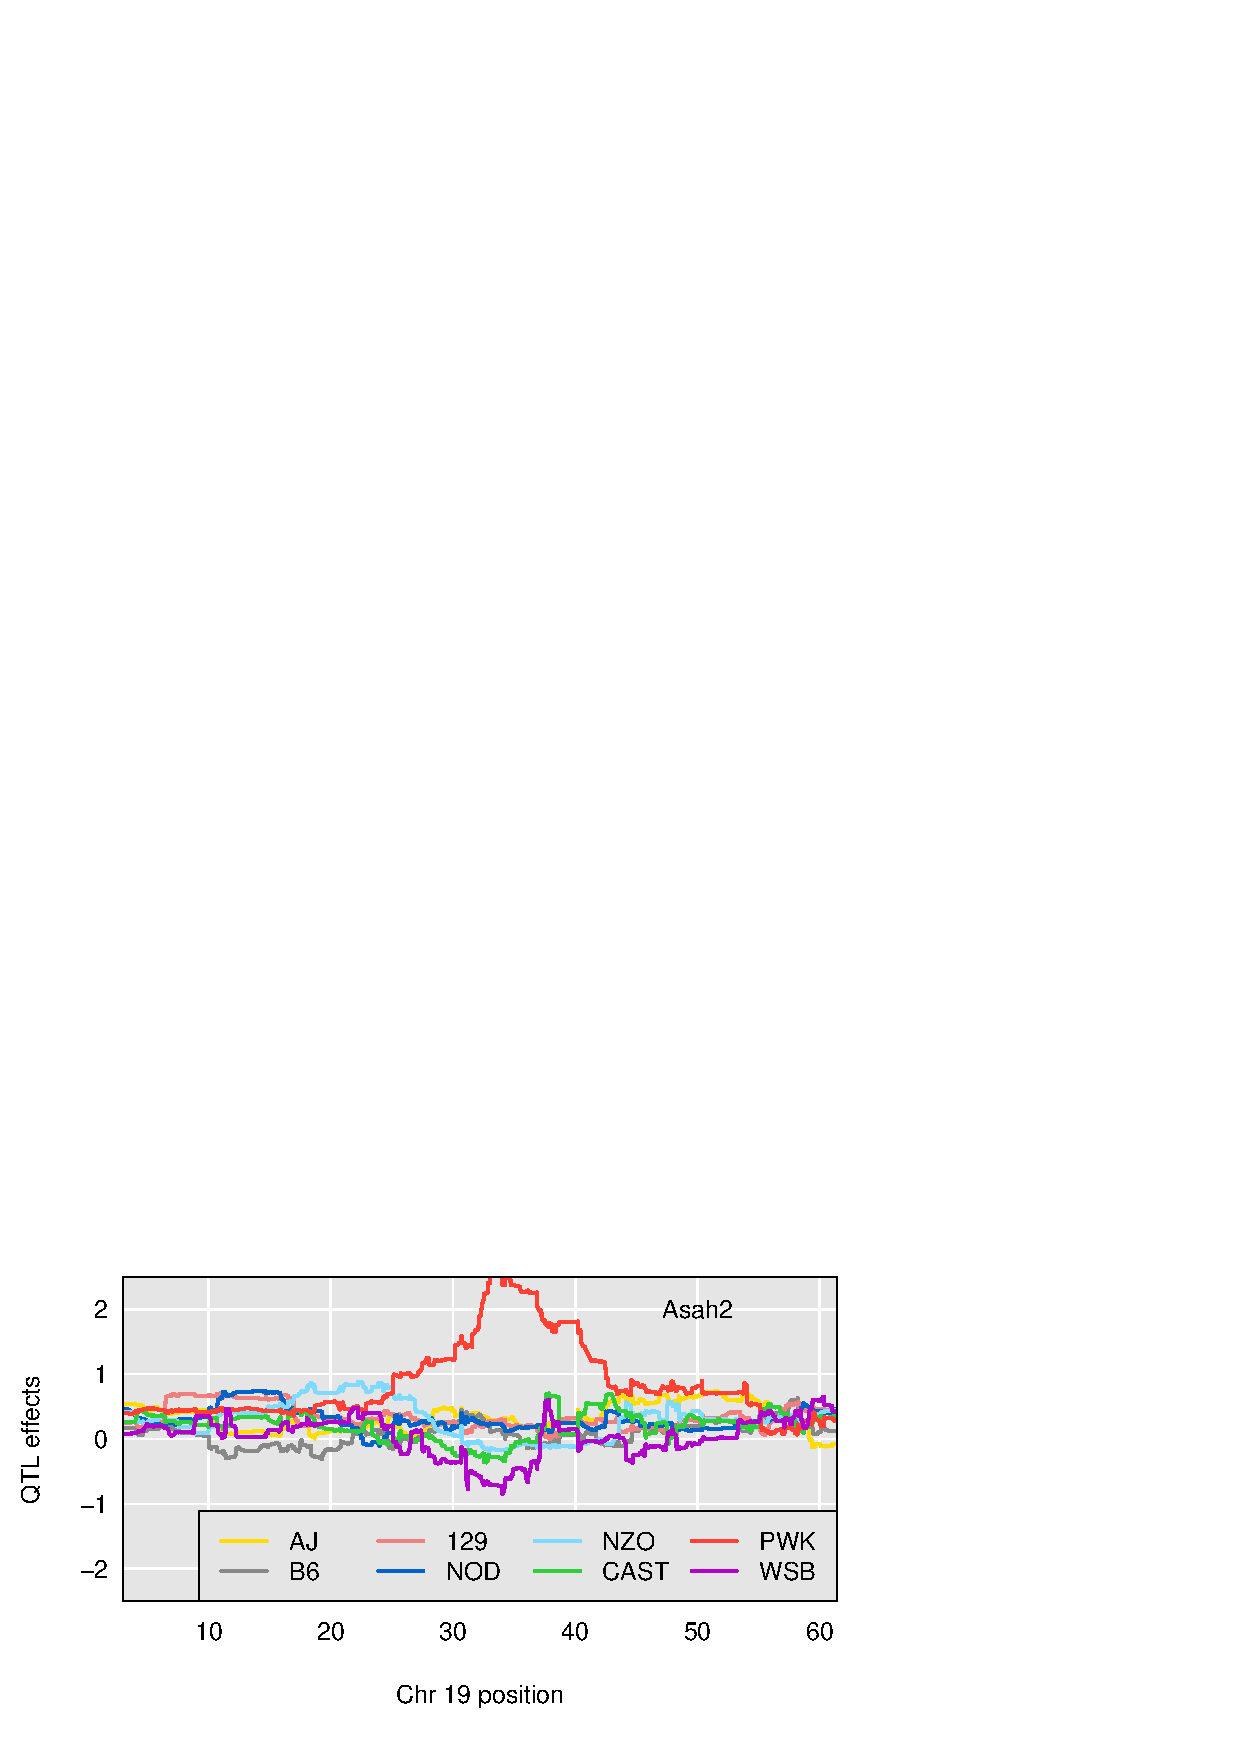
\includegraphics[width = \textwidth]{../Rmd/allele_effects_Asah2.pdf}
    \end{subfigure}%
    \begin{subfigure}[t]{0.5\textwidth}
        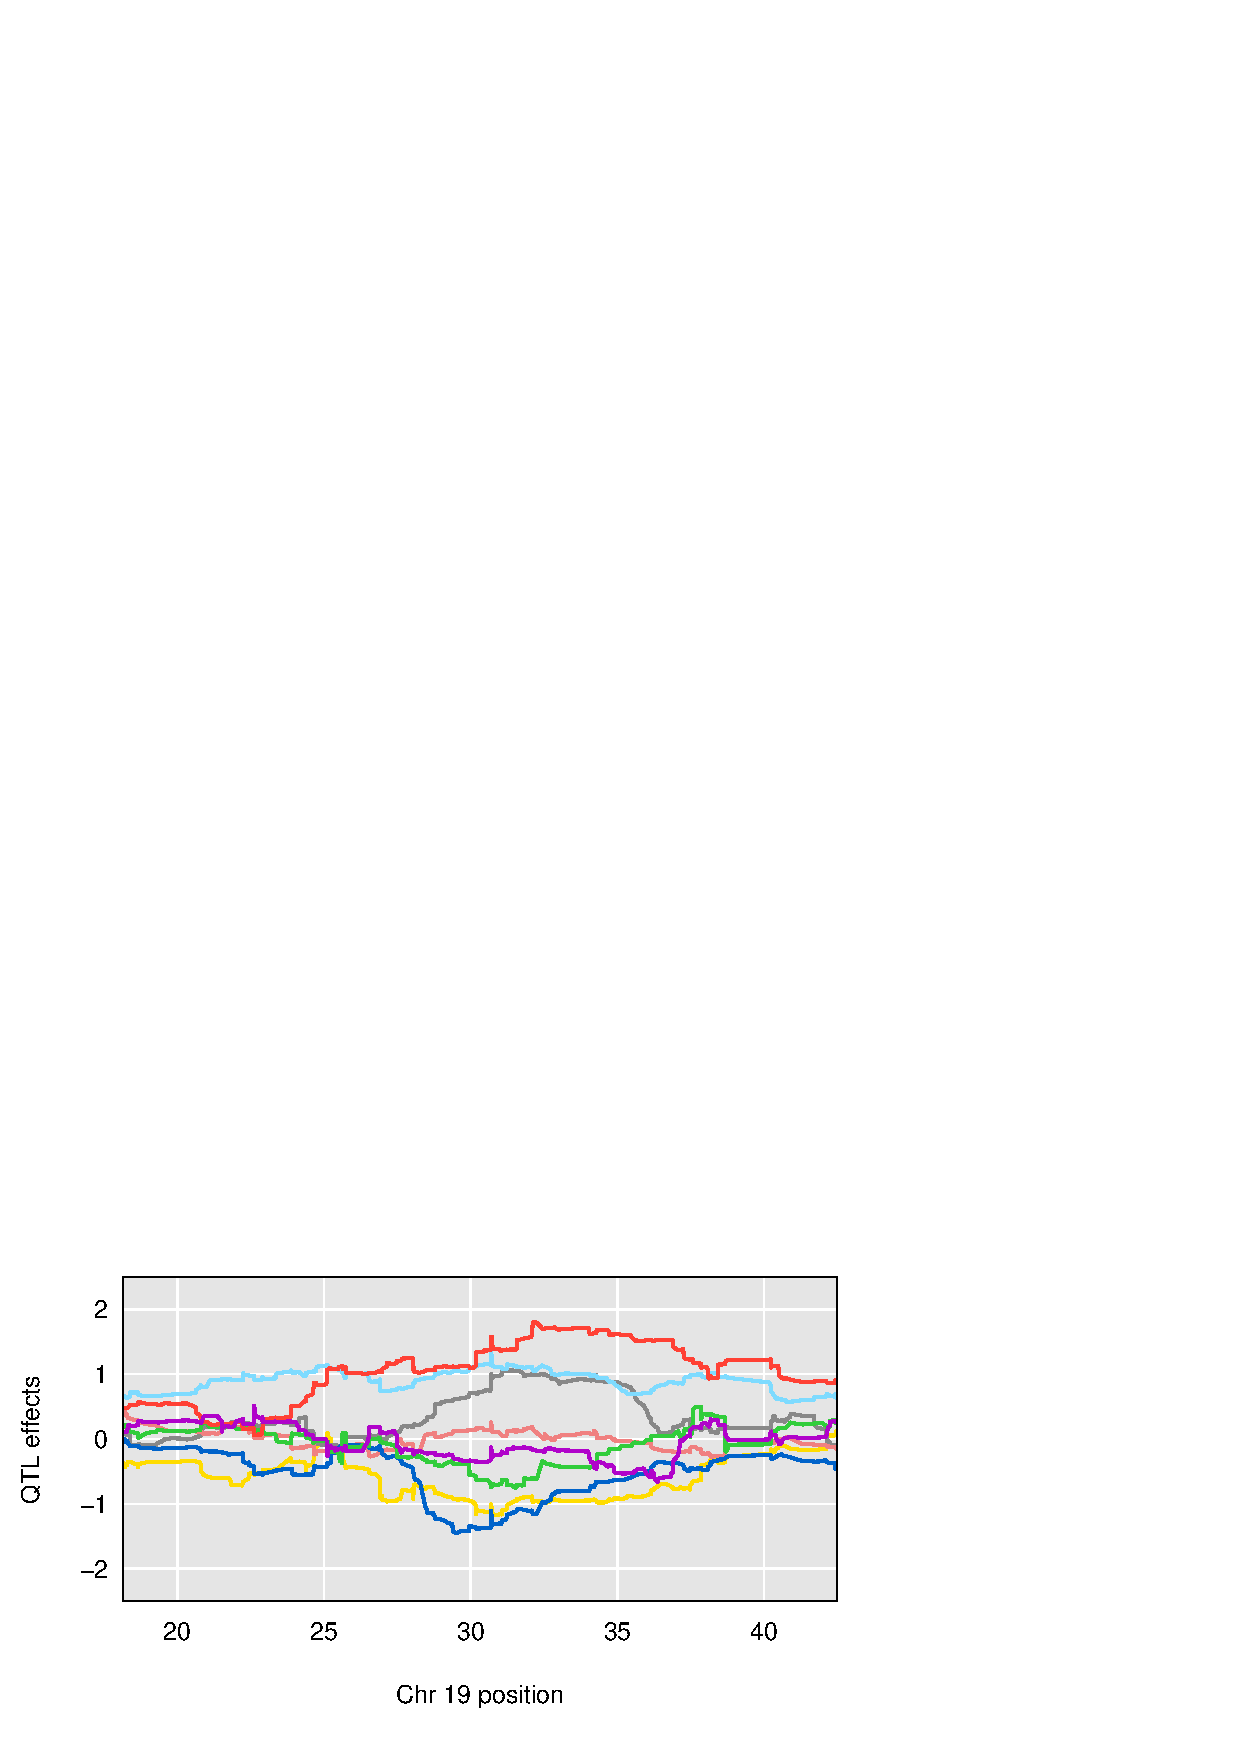
\includegraphics[width = \textwidth]{../Rmd/allele_effects_Lipo1.pdf}
    \end{subfigure}%
    
    \begin{subfigure}[t]{0.5\linewidth}
        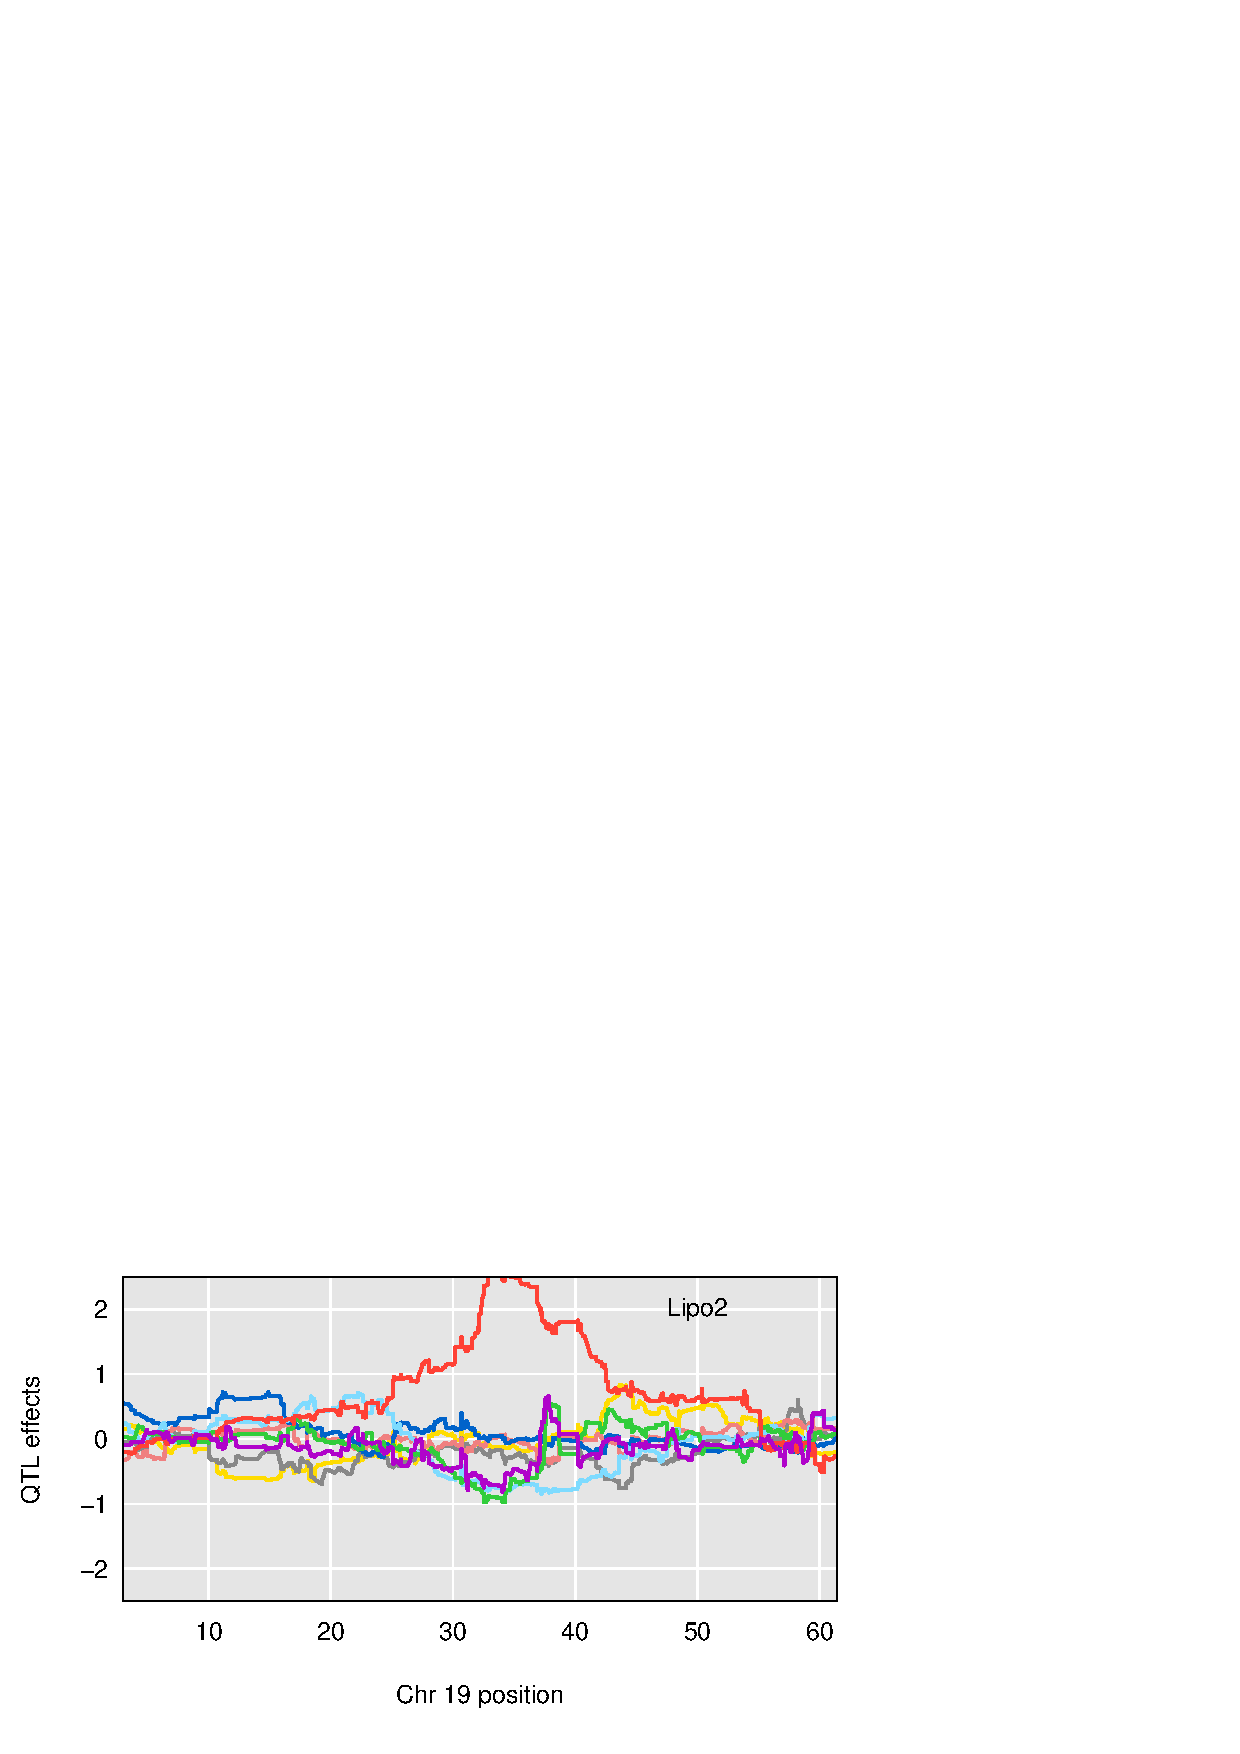
\includegraphics[width = \linewidth]{../Rmd/allele_effects_Lipo2.pdf}
    \end{subfigure}
    \begin{subfigure}[t]{0.5\linewidth}
        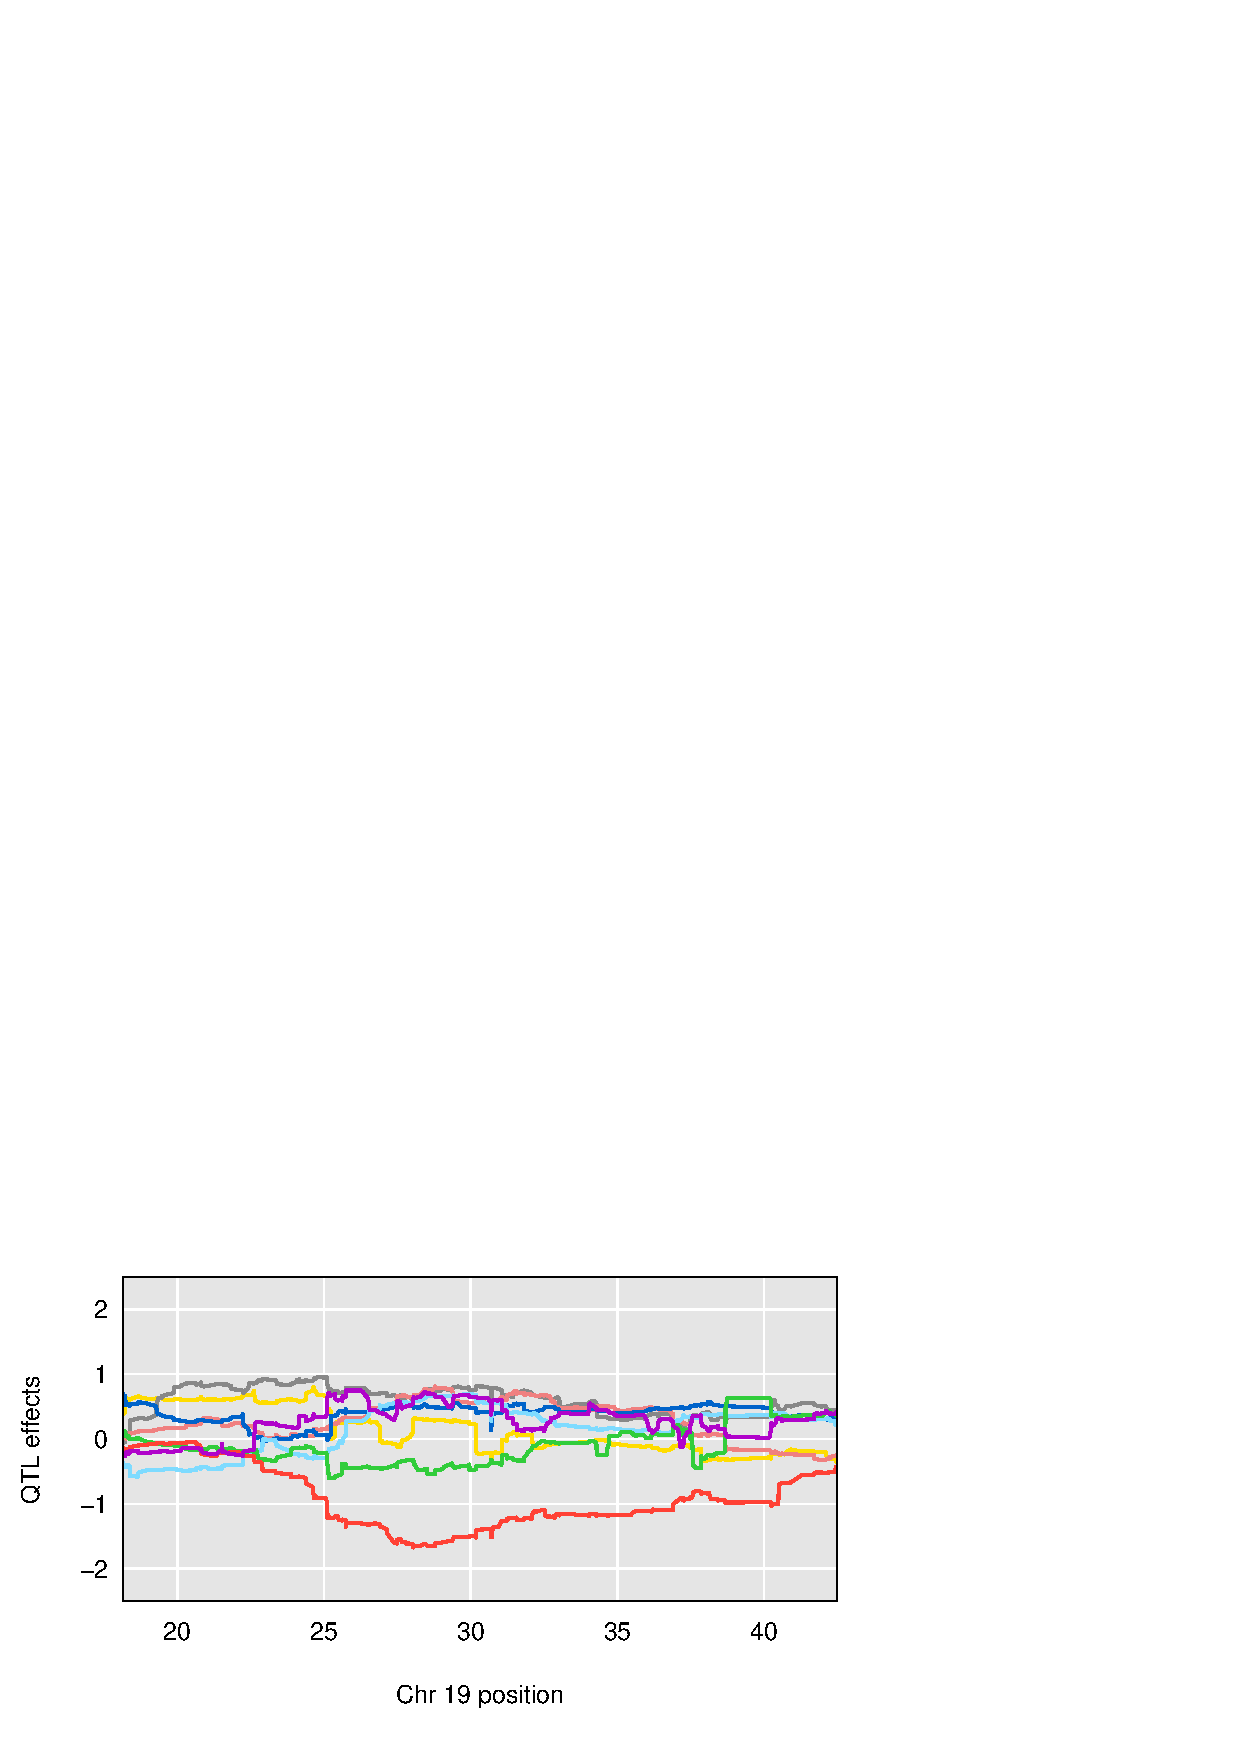
\includegraphics[width = \linewidth]{../Rmd/allele_effects_4933413C19Rik.pdf}
    \end{subfigure}
        \caption{Founder allele effects plots for Chromosome 19 for the four anchor gene expression traits reveal strong PWK effects (red) for all four traits. For \emph{Asah2} (upper left panel), WSB has a strong negative effect, opposite the direction of the PWK effect. \emph{Lipo1} (upper right panel) demonstrates NZO and B6 effects in the same direction as those of PWK, while NOD and AJ have effects in the opposite direction. The PWK peak for \emph{Lipo2} (lower left panel) demonstrates a pattern much like that of \emph{Asah2}, while the \emph{Lipo2} WSB effects are less intense than those for \emph{Asah2}. PWK and CAST have effects in the same direction for \emph{4933413C19Rik}, unlike the other genes' effects patterns.}\label{fig:founder-allele-effects}
\end{figure}

All four anchor traits demonstrate strong PWK allele effects. \emph{Lipo2} and \emph{Asah2} have nearly identical founder allele effects patterns over the two-dimensional scan region (18.1 to 42.5 Mb). 


\subsection{Pleiotropy likelihood ratio test statistic vs. chromosomal position}

\begin{figure}
    \centering
    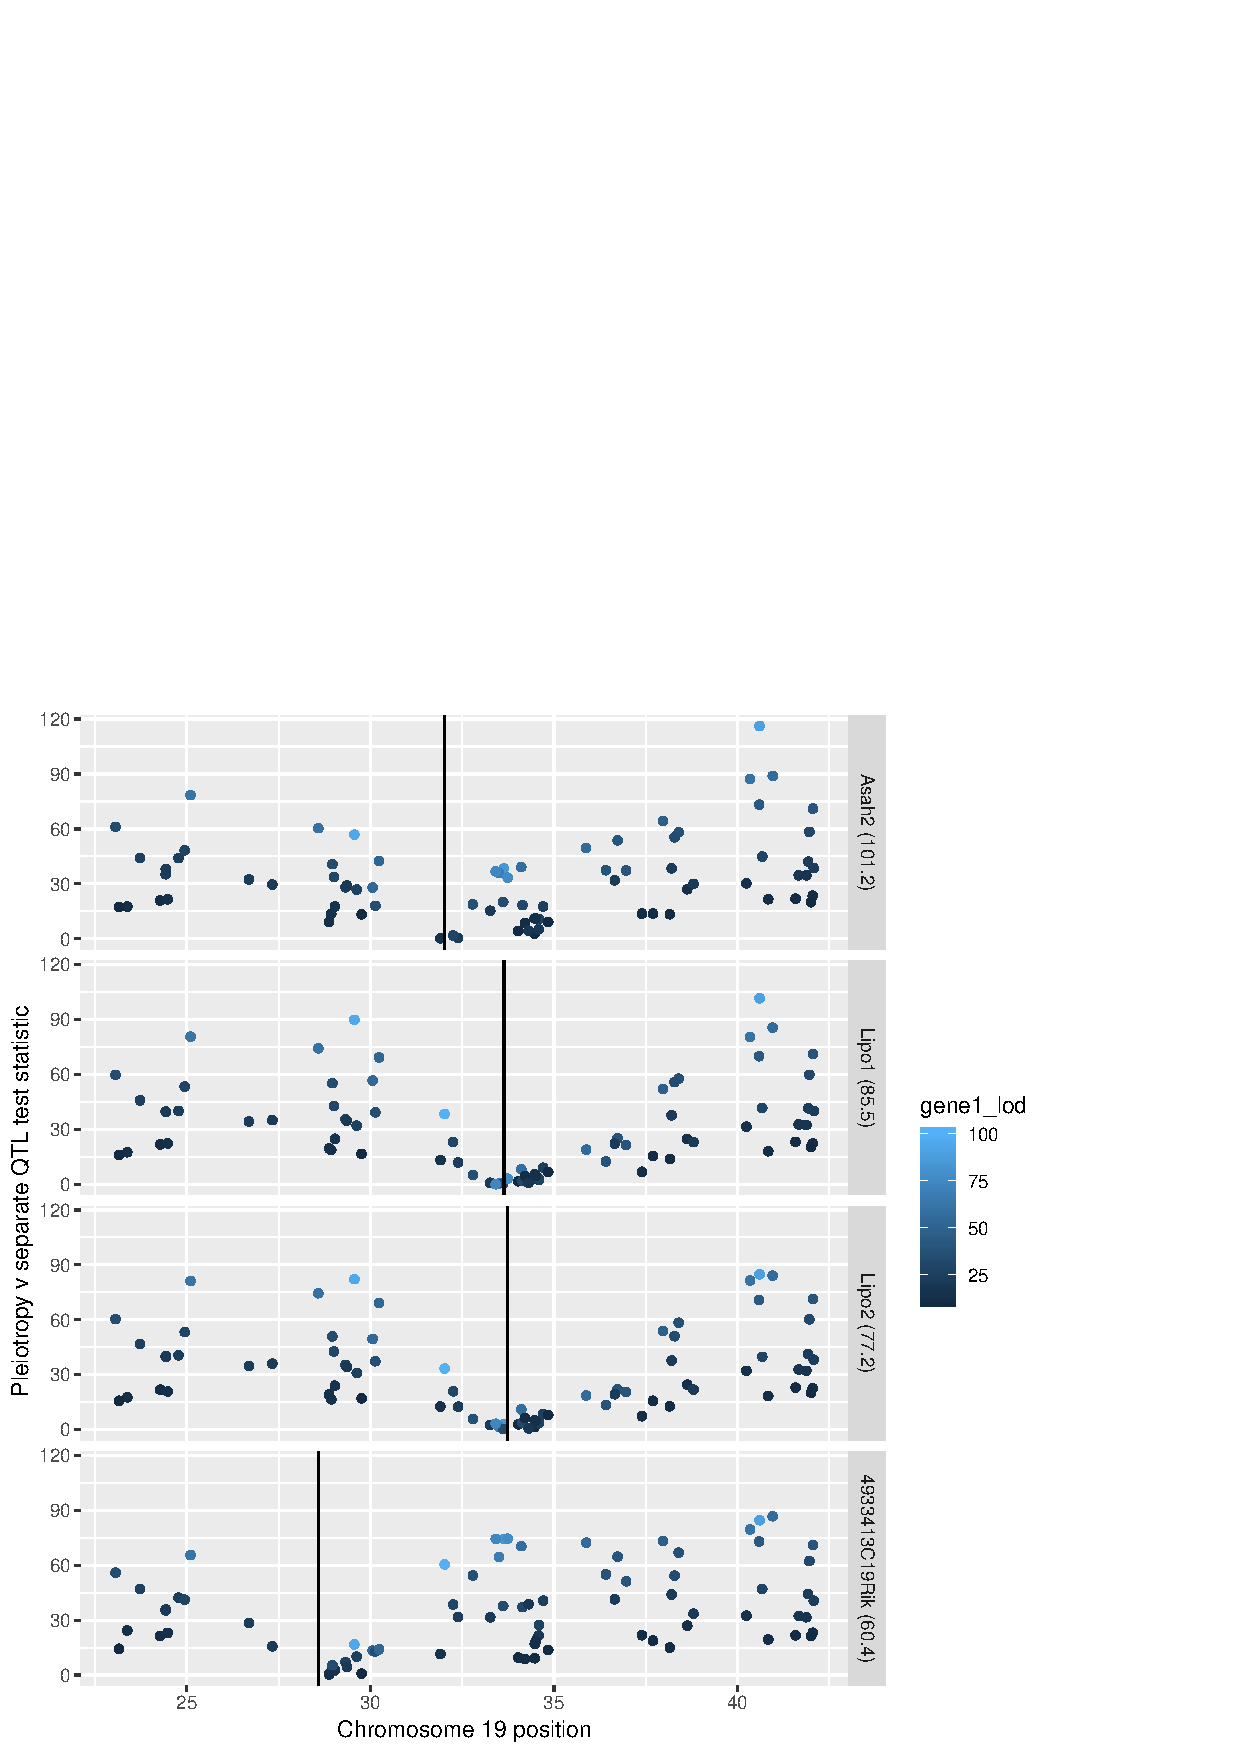
\includegraphics[width = \textwidth]{../Rmd/lrt-v-middle-of-gene.pdf}
    \caption{Each anchor gene has its own panel. Along the horizontal axis is Chromosome 19 position. The vertical axis is for pleiotropy vs. separate QTL test statistic value. Each point corresponds to a local gene expression trait. Point color corresponds to the nonlocal gene's univariate LOD peak height, with lighter shades of blue denoting greater values of univariate LOD peak height. Vertical black bar denotes the anchor gene's position on Chromosome 19. All four panels reveal that points further from the anchor gene tend to show greater test statistic values. Additionally, the Lipo1 and Lipo2 panels offer an opportunity to compare the impact of anchor gene univariate LOD peak height on pleiotropy vs. separate QTL test statistic values.}
    \label{fig:middle}
\end{figure}

Each anchor gene has its own panel in Figure \ref{fig:middle}. Along the horizontal axis is Chromosome 19 position. The vertical axis is for pleiotropy vs. separate QTL test statistic value. Each point corresponds to a local gene expression trait. Point color corresponds to the nonlocal gene's univariate LOD peak height, with lighter shades of blue denoting greater values of univariate LOD peak height. Vertical black bar denotes the anchor gene's position on Chromosome 19. All four panels reveal that points further from the anchor gene tend to show greater test statistic values. Additionally, because of their nearly identical positions, the \emph{Lipo1} and \emph{Lipo2} panels offer an opportunity to compare the impact of anchor gene univariate LOD peak height on pleiotropy vs. separate QTL test statistic values.




\subsection{Pleiotropy likelihood ratio test statistics vs. univariate LOD peak heights}

\begin{figure}
    \centering
    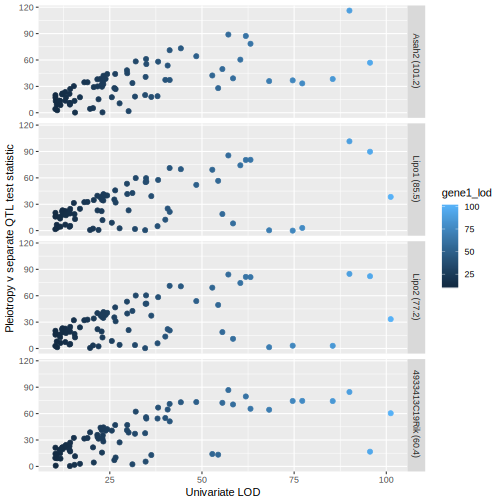
\includegraphics[width = \textwidth]{../Rmd/lrt-v-univariate-lod.pdf}
    \caption{Vertical axis denotes pleiotropy vs. separate QTL test statistic value, while horizontal axis denotes univariate LOD peak height. Each point corresponds to a single gene expression trait. Panels correspond to the anchor gene expression trait. The pleiotropy vs. separate QTL test statistics correspond to analyses involving a single gene expression trait and the specified anchor gene expression trait.}
    \label{fig:lod}
\end{figure}

Analyses for all four anchor gene expression traits demonstrate that greater univariate LOD scores tend to correspond to greater values of the pleiotropy vs. separate QTL test statistic (Figure \ref{fig:lod}). 








\subsection{Pleiotropy likelihood ratio test statistics vs. fitted values correlation}

\begin{figure}
    \centering
    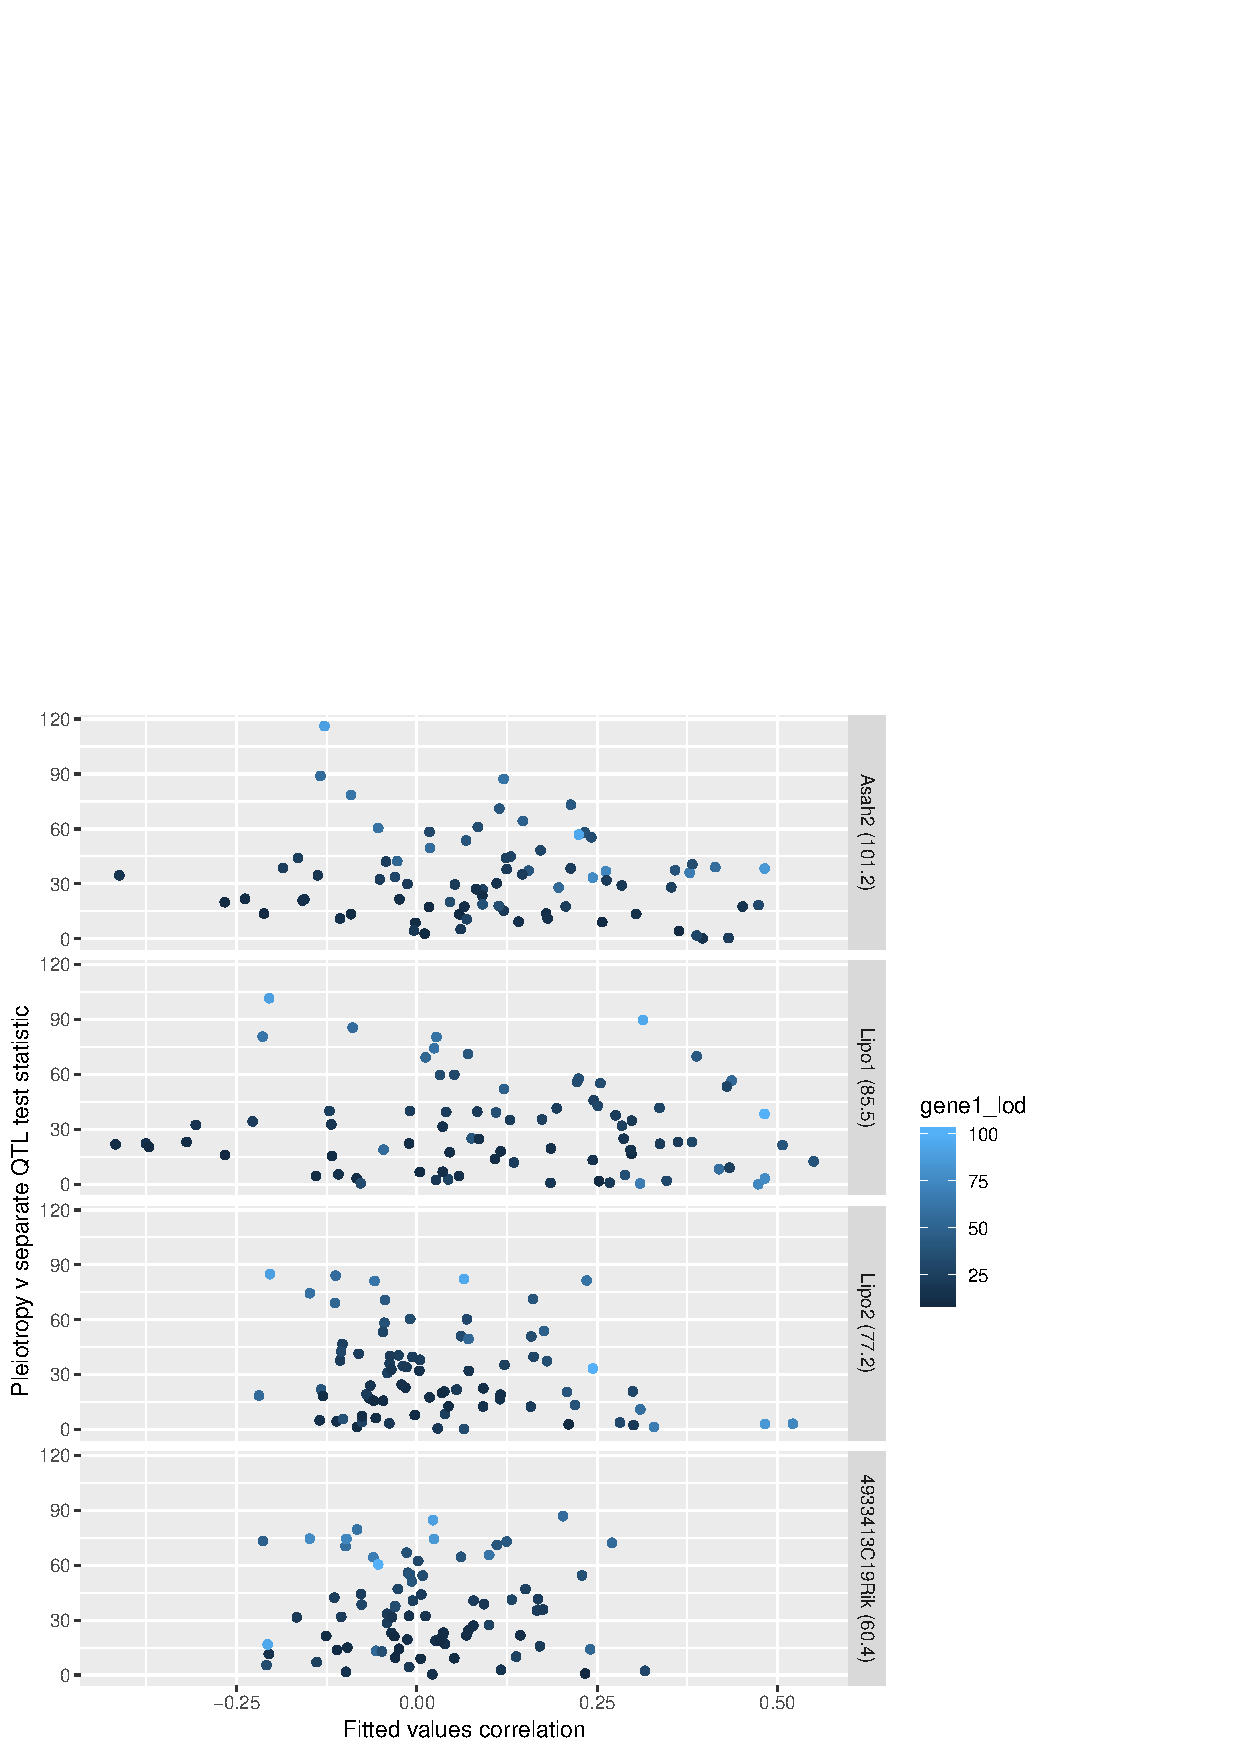
\includegraphics[width = \textwidth]{../Rmd/lrt-v-corr.pdf}
    \caption{Vertical axis denotes the pleiotropy vs. separate QTL test statistic value, and horizontal axis indicates absolute value of the correlation between vectors of fitted values. Each point corresponds to a pairing between the specified anchor expression trait and one of the 79 other expression traits.}
    \label{fig:cor}
\end{figure}

Figure \ref{fig:cor} features four panels, one for each anchor gene. Each point corresponds to a pairing between the specified anchor and one of the 79 other gene expression traits.



\section{Discussion}

Our goal for this study was to characterize the impacts of univariate LOD peak height, inter-locus distance, and founder allele effects pattern similarities on pleiotropy vs. separate QTL test statistic values. Our study design, in which we examined 310 pairs of local gene expression traits on Chromosome 19, allowed us to interrogate both the effects of univariate association strength and the effects of inter-locus distance on pleiotropy vs. separate QTL test statistic values. We found that stronger univariate associations and greater inter-locus distances correspond to greater pleiotropy vs. separate QTL test statistic values (Figures \ref{fig:middle} and \ref{fig:lod}). We expected these trends based on our simulation studies in Chapter 2.

Figure \ref{fig:cor} revealed no marginal relationship between fitted values correlations and pleiotropy vs. separate QTL test statistics. However, close examination of Figure \ref{fig:cor} reveals the possibility that there is an interaction between 1) fitted values correlations and 2) univariate association strength. In every panel, those expression traits with stronger univariate associations tend to have steeper slopes between the conditional mean pleiotropy test statistic values and fitted values correlations. The plots suggest that, at greater univariate LOD values, there is a greater (negative) relationship between fitted values correlation and pleiotropy vs. separate QTL test statistic value. 

We anticipated that more similar founder allele effects patterns would correspond to smaller values for the pleiotropy vs. separate QTL test statistic, when holding other factors constant. As we stated above, \citet{macdonald2007joint} and \citet{king2012genetic} argued that, for biallelic markers, two pleiotropic traits should have similar founder allele effects patterns. In our setting, it's unclear whether the markers are biallelic in the collection of eight founder lines. 

We've demonstrated strong evidence in support of the roles of 1) univariate QTL LOD peak heights and 2) interlocus distances impacting pleiotropy vs. separate QTL test statistic values. Greater univariate QTL peak heights and greater interlocus distance lead to greater pleiotropy vs. separate QTL test statistics. Future research may clarify the impoact of founder allele effects patterns on pleiotropy vs. separate QTL test statistics. The fact that all four anchor traits had strong PWK effects limited our ability to fully define the impact of allele effects patterns on our test statistics.

Throughout this study, we elected to use test statistic values rather than p-values, as our measure of evidence supporting the separate QTL hypothesis. The primary reason for doing this is to avoid the computationally costly bootstrap sampling and two-dimensional QTL scans that we would need to get bootstrap p-values.

We share our analysis \texttt{R} code \citep{r} as a \texttt{git} repository at this URL: \url{https://github.com/fboehm/keller-2018-chr19-power}.



\printbibliography


% latex table generated in R 3.5.2 by xtable 1.8-3 package
% Thu Jan  3 16:43:33 2019
\begin{table}[ht]
\centering
\begingroup\tiny
\begin{tabular}{>{\em}lrrrr}
  \hline
symbol & start & end & peak\_position & lod \\ 
  \hline
C030046E11Rik & 29.52 & 29.61 & 29.55 & 95.58 \\ 
  Tctn3 & 40.60 & 40.61 & 40.59 & 90.00 \\ 
  Gm7237 & 33.41 & 33.42 & 33.67 & 74.61 \\ 
  Lipo4 & 33.50 & 33.52 & 34.00 & 68.23 \\ 
  Dock8 & 25.00 & 25.20 & 25.07 & 63.17 \\ 
  Sorbs1 & 40.30 & 40.40 & 40.48 & 61.89 \\ 
  Lipm & 34.10 & 34.12 & 34.06 & 58.43 \\ 
  Blnk & 40.93 & 40.99 & 40.76 & 57.16 \\ 
  A830019P07Rik & 35.84 & 35.92 & 35.60 & 55.54 \\ 
  Uhrf2 & 30.03 & 30.09 & 29.96 & 54.40 \\ 
  Mbl2 & 30.23 & 30.24 & 30.18 & 52.81 \\ 
  Myof & 37.90 & 38.04 & 38.05 & 48.46 \\ 
  Gm27042 & 40.59 & 40.59 & 40.61 & 44.27 \\ 
  Btaf1 & 36.93 & 37.01 & 36.90 & 41.25 \\ 
  Hoga1 & 42.05 & 42.07 & 42.09 & 41.23 \\ 
  Ppp1r3c & 36.73 & 36.74 & 36.53 & 40.69 \\ 
  Pcgf5 & 36.38 & 36.46 & 36.24 & 40.06 \\ 
  Slc35g1 & 38.40 & 38.41 & 38.35 & 38.11 \\ 
  Pten & 32.76 & 32.83 & 32.77 & 37.95 \\ 
  Gldc & 30.10 & 30.18 & 30.17 & 36.26 \\ 
  Lgi1 & 38.26 & 38.31 & 38.17 & 34.91 \\ 
  C330002G04Rik & 23.04 & 23.08 & 23.34 & 34.84 \\ 
  Ppapdc2 & 28.96 & 28.97 & 29.09 & 34.71 \\ 
  Gm8978 & 33.61 & 33.63 & 33.03 & 34.59 \\ 
  Mms19 & 41.94 & 41.98 & 41.98 & 32.03 \\ 
  Ankrd22 & 34.12 & 34.17 & 34.04 & 31.83 \\ 
  Cdc37l1 & 28.99 & 29.02 & 29.03 & 31.14 \\ 
  Sgms1 & 32.12 & 32.39 & 32.11 & 30.10 \\ 
  Entpd1 & 40.61 & 40.74 & 40.50 & 29.73 \\ 
  Cbwd1 & 24.92 & 24.96 & 24.73 & 29.65 \\ 
  Gm14446 & 34.59 & 34.60 & 34.28 & 27.65 \\ 
  Ermp1 & 29.61 & 29.65 & 29.70 & 26.57 \\ 
  Gm9938 & 23.72 & 23.73 & 23.87 & 26.46 \\ 
  Insl6 & 29.32 & 29.33 & 29.37 & 26.23 \\ 
  Slc16a12 & 34.67 & 34.75 & 34.71 & 25.54 \\ 
  Pgm5 & 24.68 & 24.86 & 25.00 & 24.30 \\ 
  Morn4 & 42.07 & 42.09 & 41.79 & 23.86 \\ 
  Exosc1 & 41.92 & 41.93 & 42.10 & 23.28 \\ 
  Smarca2 & 26.61 & 26.78 & 26.59 & 23.25 \\ 
  4930418C01Rik & 24.42 & 24.43 & 23.92 & 23.10 \\ 
  2700046G09Rik & 32.39 & 32.39 & 32.25 & 23.02 \\ 
  Kcnv2 & 27.32 & 27.34 & 27.14 & 22.88 \\ 
  1500017E21Rik & 36.61 & 36.71 & 37.07 & 22.78 \\ 
  Fra10ac1 & 38.19 & 38.22 & 38.35 & 22.48 \\ 
  Rnls & 33.14 & 33.39 & 34.17 & 21.94 \\ 
  Noc3l & 38.79 & 38.82 & 40.20 & 21.67 \\ 
  Pip5k1b & 24.29 & 24.56 & 24.15 & 21.62 \\ 
  Plgrkt & 29.35 & 29.37 & 29.37 & 20.65 \\ 
  Ifit3 & 34.58 & 34.59 & 34.28 & 20.45 \\ 
  Fas & 34.29 & 34.33 & 34.20 & 19.65 \\ 
  Slit1 & 41.60 & 41.74 & 41.70 & 18.95 \\ 
  Rrp12 & 41.86 & 41.90 & 41.71 & 18.09 \\ 
  Ak3 & 29.02 & 29.05 & 29.55 & 16.90 \\ 
  A1cf & 31.87 & 31.95 & 32.11 & 15.56 \\ 
  4430402I18Rik & 28.90 & 28.97 & 29.37 & 15.43 \\ 
  Pdlim1 & 40.22 & 40.27 & 40.25 & 15.25 \\ 
  Gm26902 & 34.47 & 34.48 & 36.15 & 14.26 \\ 
  Plce1 & 38.48 & 38.79 & 38.42 & 14.26 \\ 
  Slc1a1 & 28.84 & 28.91 & 28.97 & 14.18 \\ 
  Fam122a & 24.48 & 24.48 & 24.08 & 14.07 \\ 
  Lipa & 34.49 & 34.53 & 34.29 & 14.06 \\ 
  Mamdc2 & 23.30 & 23.45 & 23.35 & 13.12 \\ 
  Kif11 & 37.38 & 37.42 & 37.33 & 12.93 \\ 
  4933411K16Rik & 42.05 & 42.05 & 42.08 & 12.92 \\ 
  Ccnj & 40.83 & 40.85 & 40.59 & 12.19 \\ 
  Gm340 & 41.58 & 41.59 & 41.30 & 12.17 \\ 
  Fxn & 24.26 & 24.28 & 24.31 & 12.07 \\ 
  Stambpl1 & 34.19 & 34.24 & 34.28 & 11.62 \\ 
  Pde6c & 38.13 & 38.18 & 38.07 & 11.54 \\ 
  Cyp26a1 & 37.70 & 37.70 & 37.48 & 11.35 \\ 
  Ch25h & 34.47 & 34.48 & 32.50 & 10.74 \\ 
  Pank1 & 34.81 & 34.88 & 35.55 & 10.61 \\ 
  9930021J03Rik & 29.71 & 29.81 & 28.71 & 10.32 \\ 
  Klf9 & 23.14 & 23.17 & 23.34 & 10.26 \\ 
  Ubtd1 & 41.98 & 42.03 & 41.71 & 10.25 \\ 
  Lipk & 34.01 & 34.05 & 34.29 & 10.23 \\ 
   \hline 
\end{tabular}
\endgroup
\caption{Annotations for 76 non-anchor genes on Chromosome 19.}\label{tab:ann76}
\end{table}

\end{document}
